\documentclass[../main.tex]{subfiles}
\chapter{Validierung}
\label{c:validierung}

Die Beschreibung der Maschinenkinematik erfolgt mit einer homogenen Transformationsmatrix je Freiheitsgrad.
Die der Simulation zugrunde liegende Maschine hat sechs geführte Freiheitsgrade.
Von diesen sind vier über einen Vorschub an die Drehzahl des Werkzeugs gekoppelt.
Die positive Richtung dieser Freiheitsgrade ist außerdem nicht streng anhand der mathematisch positive Richtung des Standardkoordinatensystems definiert.

Um Vorzeichen- und Drehmittelpunktfehler sowie Fehler in der Anwendungsreihenfolge der Abbildungsmatrizen zu erkennen, ist eine qualitative und visuelle Validierung der in Kap.\ \ref{c:herleitung} entwickelten linearen Algebra anhand einer erprobten Methode sinnvoll.
Diese Methode sollte Teil der \matlab-Toolchain sein, erlauben das Modell extern zu bedaten und eine grafische Ausgabe zur Verfügung stellen.

Aufgrund der direkten Schnittstelle zu \matlab wurde entschieden das kinematische Modell als \simscape Multibody Modell aufzubauen.
,,Bei \simscape handelt es sich um eine Reihe von Blockbibliotheken und speziellen Simulationsfunktionen zur Modellierung physikalischer Systeme in der \simulink-Umgebung.
Sie verwendet den Physical Network-Ansatz, der sich von dem Standard \simulink Modellierungsansatz unterscheidet und sich besonders für die Simulation von Systemen eignet, die aus realen physikalischen Komponenten bestehen.'' \cite[aus dem Englischen übersetzt]{mwSim}.

Vergleichbar zu \simulink wird hier ein Signalflussplan erstellt, der die Wechselwirkung von Funktionsgruppen mit Hilfe von Verbindungen beschreibt.
Diese Verbindungen stellen in \simulink Signale dar, üblicherweise zeitdiskrete Zahlenwerte oder logische Zustände.
In \simscape repräsentieren diese Verbindungen allerdings die Position und Ausrichtung eines Koordinatensystems im Raum.
Das Signal übertragt also die Information über die Transformation von einem Referenzsystem zu einem Zielsystem.

Die verschiedenen Formen der Modellierung von \simulink uns \simscape können in einem Blockschaltbild koexistieren und mit Hilfe von ,,Physical Signal Converters'' vereint werden.
So kann ein \simulink-Signal in eine zeitdiskrete Transformation eines Koordinatensystem gewandelt werden, oder Position und Ausrichtung eines Koordinatensystems in einem Signal erfasst werden.

\section{Mechanisches Modell der Maschine}

Anhand der schematischen Darstellung einer Wälzfräsmaschine in Abb.\ \ref{fig:maschine} wurde in Creo Parametric ein dreidimensionales Modell erstellt.
Die Komponenten der Maschine wurden im Mechanismus-Modus zu einem kinematischen Modell verknüpft.
Dieses kinematische CAD-Modell wurde anschließend mittels einer Softwareschnittstelle in ein \simscape Multibody Modell konvertiert.

Ursprung des CAD-Modells ist das Maschinenbett-Koordinatensystem.
Anfänglich wurden alle Komponenten der Maschine auf dieses Standard-Koordinatensystem konstruiert.
Nach Konvertierung der CAD-Komponenten in ein neutrales Datenformat beinhalten alle Teile dieses Koordinatensystem als Ursprung.
Dadurch sollte der Aufbau des \simscape Modells vereinfachen werden, da alle Komponenten ohne linearen oder rotatorischen Versatz auf des world-Koordinatensystem referenziert werden können.
Das world-Koordinatensystem ist raumfest (siehe Abschnitt \ref{c:homtransform}) und als solches das Bezugssystem für das Simulationsmodel.

\begin{figure}
	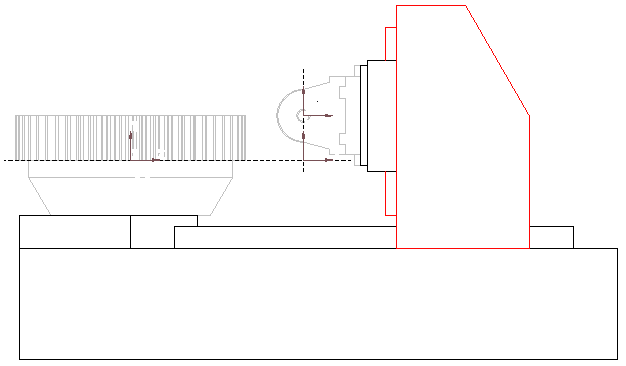
\includegraphics{skelettmodell}
	\caption{Konstruktion des Koordinatensystems für Schlitten in x-Richtung}
	\label{fig:skelettmodell}
\end{figure}

Die in \simscape zur Verfügung stehenden Joint-Blöcke verwenden als primäre Achse allerdings immer die z-Achse.
Translationen können ausschließlich entlang der z-Achse erfolgen und Rotationen erfolgen entsprechend ausschließlich um die z-Achse.
Es ist somit notwendig, den Komponenten zweckmäßige und individuelle Koordinatensysteme aufzuprägen statt alle auf ein gemeinsames Ursprungs-Koordinatensystem zu referenzieren.

Eine Möglichkeit ist es, dass dies direkt im CAD-Modell geschieht und das Bauteil mit individuellem Bezugssystem exportiert wird.
Häufig müssen Bauteile jedoch zwei Koordinatensysteme haben, eines als ihr eigener Ursprung und ein weiteres, welches sie an ein Tochterbauteil in der kinematischen Kette vererben können.
In \simscape besteht deswegen eine andere Möglichkeit innerhalb eines ,,File Solid'' Blocks eine Koordinatentransformation zu definieren.
Mechanische Komponente können in \simscape mit einem ,,File Solid'' Block repräsentiert werden, wenn die Geometrie aus externen Daten geladen wird.
Dieser Block hat, wie andere mechanische Blöcke, einen Koordinatensystem-Eingang und es können transformierte Koordinatensysteme als Ausgänge ergänzt werden.
Maskiert innerhalb des Blockes wird so eine feste, zeitinvariante Transformation von Eingang- zu Ausgangskoordinatensystem definiert.
Die Möglichkeiten ein solches sekundäres Koordinatensystem zu definieren sind begrenzt.
So können lediglich ein Koordinatensystem, der Massenschwerpunkt des Körpers sowie der Flächenschwerpunkt einer frei wählbaren Fläche als Ursprung dienen, nicht etwa ein definierbarer Punkt im Raum.
Es ist somit notwendig, die Konstruktion dieser Ketten von Koordinatensystem geschickt anzugehen.

In Abbildung \ref{fig:skelettmodell} ist die Konstruktion des Koordinatensystems für den Maschinenschlitten der X-Achse in roter Umrandung dargestellt.
Als Ursprung für das Koordinatensystems $\{b\}$ bietet sich der Schnittpunkt von Hauptachsen der Koordinatensysteme $\{a\}$ und $\{c\}$ an.
So kann das Koordinatensystem $\{c\}$, unabhängig der gewählten Ausrichtung von $\{b\}$, entlang einer der Hauptachsen von $\{b\}$ liegen.
Somit wird keine weitere Transformation innerhalb der betrachteten Komponente notwendig.
Die Ausrichtung von $\{b\}$ sollte so gewählt werden, dass die z-Achse direkt in positive Richtung der linearen Maschinenachse geht.
Dieser einachsige, translatorische Freiheitsgrad wird mit einem Joint-Block modelliert.
Das Koordinatensystem $\{c\}$ ist wiederum translatorisch verschoben, sodass der Ursprung auf der Rotationsachse der Werkzeugspindel liegt.
Im Modell ist $\{c\}$ das Koordinatensystem des in der kinematischen Kette nachfolgend liegenden Teiles, der Schlitten der Maschinen-Z-Achse.
Dieses muss im nächsten Schritt gedreht werden, sodass die z-Achse in Richtung der Rotationsachse der A-Achse zeigt.

\section{Aufbau des Simscape Multibody Modells}

\begin{figure}
	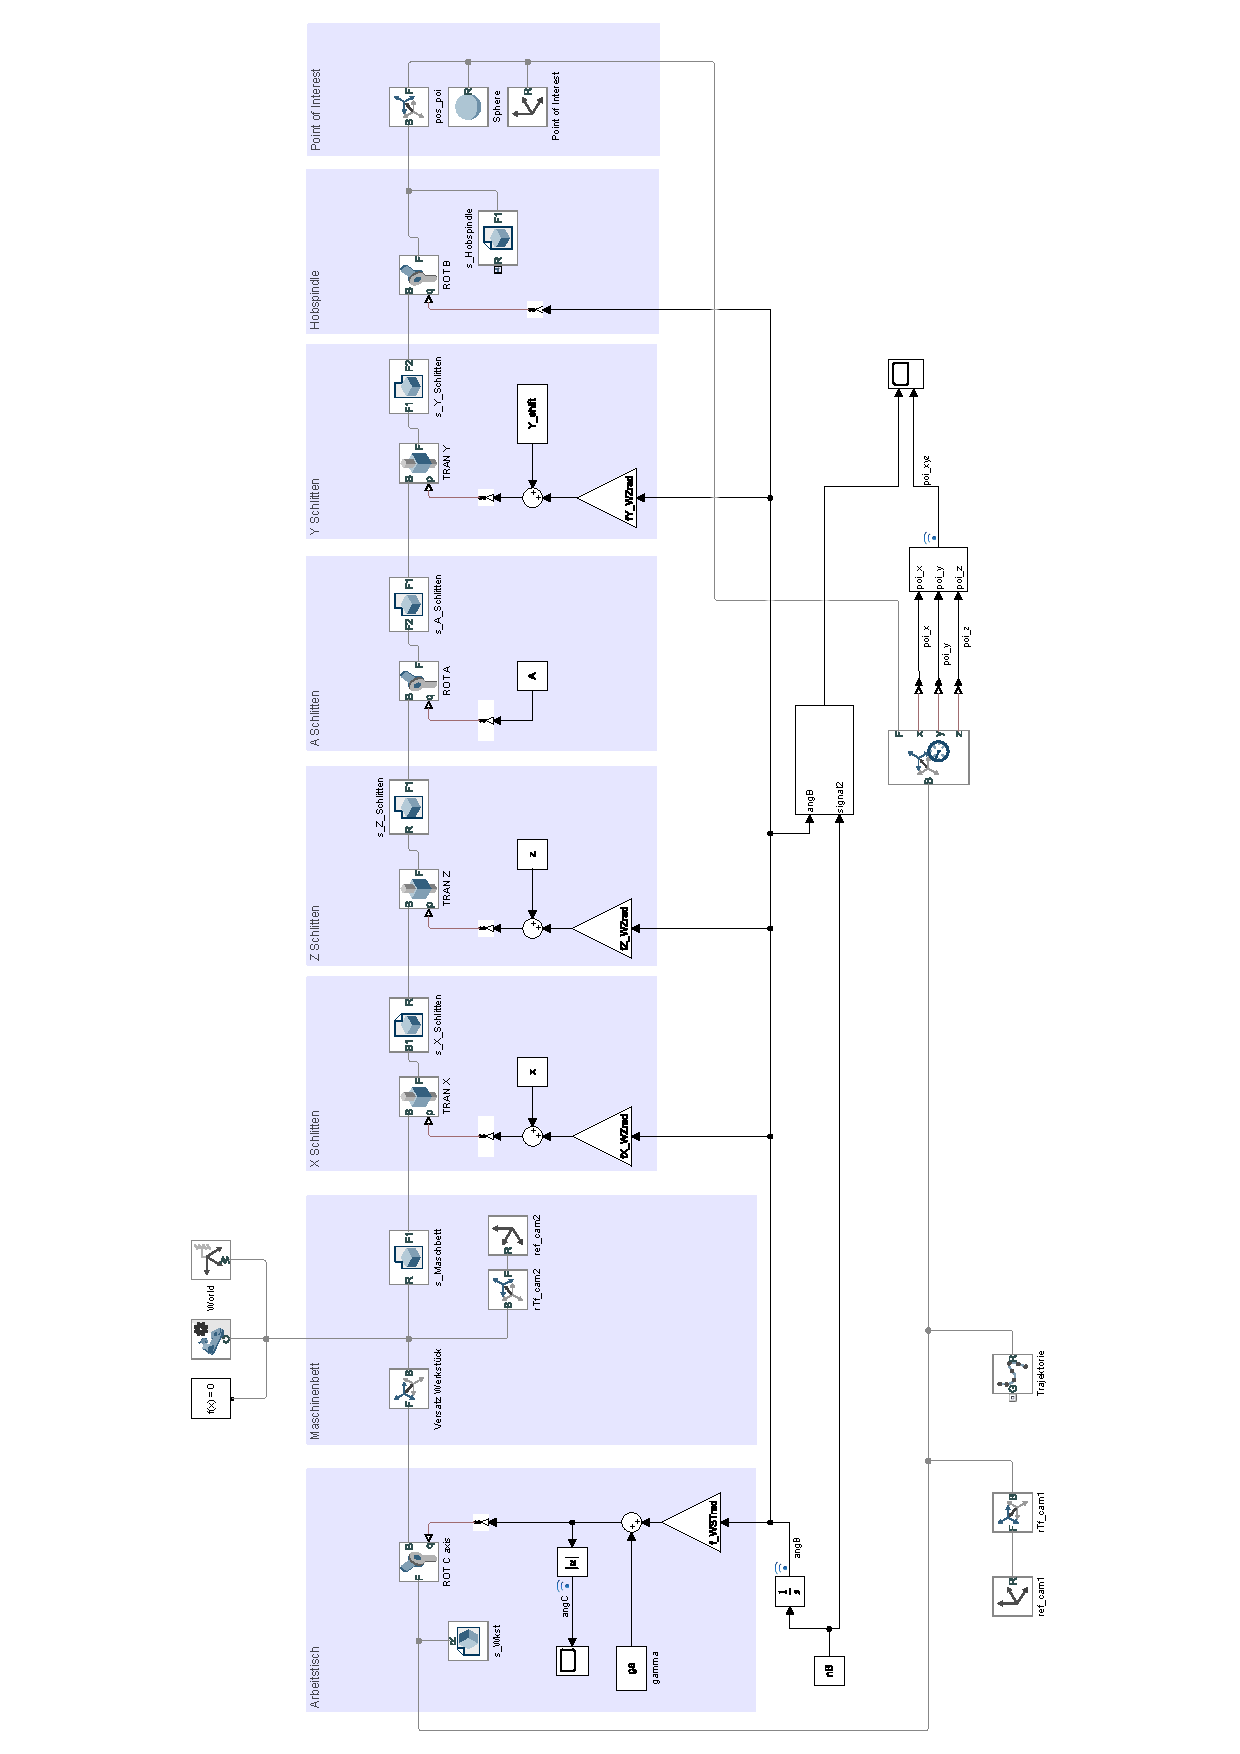
\includegraphics[scale=0.75]{simscapemdl}
	\caption{Signalflussplan des \simscape Modells}
	\label{fig:simscapemdl}
\end{figure}

Abbildung \ref{fig:simscapemdl} zeigt den Signalflussplan des zur Validierung eingesetzten \simscape Modells.
Ausgehend vom Ursprung des Modells, des ,,world''-Koordinatensystems, breiten sich die gleichen zwei Pfade aus, die in \ref{c:maschkinematik} bereits beschrieben wurden.

Im Werkstück-Pfad muss zunächst der Versatz des Bearbeitungstisches berücksichtigt werden.
Dies erfolgt mit einem ..Rigid Transform'' Block, welcher dem Signal eine Translation aufprägt, vgl. Gleichung \ref{eq:translation}.
Die Werte der Translation werden zu Laufzeit aus dem Basis-Workspace von \matlab eingelesen.

Die Funktionsweise des Bearbeitungstisches wird mit einem ,,Revolute Joint'' Block realisiert.
Blöcke der Klasse ,,Joint'' konvertierten das Signal ausgehend vom Base-Frame, dem Eingang, zum Follower-Frame, dem Ausgang, entlang spezifischen Freiheitsgraden und können über Ports mit Führungsgrößen beaufschlagt werden.
Die Zielgrößen sind Position und Geschwindigkeit, den Blöcken können jedoch ebenfalls Kräfte aufgeprägt werden.
Die resultierend notwendigen Berechnungen von Geschwindigkeit und Position bei Vorgabe einer Kraft, sowie umgekehrt die zum Erreichen einer vorgegebenen Position oder Geschwindigkeit erforderlichen Kräfte werden innerhalb des Simscale Blocks durchgeführt und können über einen Port zurückgegeben werden.
Die vorliegende Simulation beschäftigt sich nicht mit den auftretenden Kräften, sie bleiben somit unberücksichtigt.
Beim Revolute Joint sind alle Freiheitsgrade außer Rotation um die z-Achse gesperrt.

Den dynamischen Zusammenhängen zugrunde liegt der Winkel des Werkzeuges in Folge der Werkzeugrotation.
Er wird berechnet durch Integration der Drehzahl unter der Annahme, dass diese in Bogenmaß pro Zeit definiert ist.

Im Falle der C-Achse wird dieser Winkel gemäß Gleichung \ref{eq:wrkstwinkel} mit dem Vorschubfaktor multipliziert und der Offset $\gamma$ addiert.
Bei der Integration der Werkzeugdrehung wird der konstante Faktor $\feed{C}{WSt}$, der eigentlich das Verhältnis von Werkzeugdrehzahl und Werkstückdrehzahl beschreibt, vor die Integration gezogen.
Er kann dann in gleichem Maße zur Berechnung des Werkstückwinkels aus dem Werkzeugwinkel verwendet werden.
Das Ergebnis wird mit einem ,,Simulink-PS Converter'' in ein Physical Signal konvertiert und dem Revolute Joint als Positionsziel vorgegeben.

Im Werkzeugpfad wird zunächst innerhalb des Maschinenbettes (File Solid Block) das Koordinatensystem gedreht, sodass der folgende Prismatic Joint der Maschinen-X-Achse entlang der z-Achse wirken kann.
Durch Multiplikation des Werkzeugwinkels mit dem Vorfaktor $\feed{X}{Wz}$, der die Einheit $\left[\si{\milli\meter\per\radian}\right]$ hat, und Addition eines Offsets gemäß Gleichung \ref{eq:xaxisfun} erhalten wir den Wert der Translation.
Dieser wird wieder konvertiert und dem Block als Positionsziel vorgegeben.
In Folge wird der File Solid Block mit dem Maschinen-X-Schlitten geschaltet.
In diesem erfolgt die Transformation des Koordinatensystems, sodass z-Achse parallel zur Maschinen-Z-Achse ist.
Der Block ist in diesem Fall so eingebaut, dass das aus dem CAD-Skelettmodell stammende Koordinatensystem als Ausgang verwendet wird und somit in Richtung des folgenden Freiheitsgrades zeigt.
Es muss deswegen ein transformiertes Koordinatensystem konstruiert werden, das parallel zu dem aus dem Maschinenbett übergebenen Koordinatensystem liegt und als Eingang in den Block definiert werden.

Zur Modellierung der folgenden Freiheitsgrade wurde sich bei Strategien der bisher beschrieben Modellausschnitte bedient.
Am Ende der kinematischen Kette erhält man das Werkzeugkoordinatensystem in welches der betrachtete Punkt, Point of Interest (PoI), konstruiert werden kann.
Durch Verschieben des Ursprungs um die Koordinaten des Punktes, welche aus dem Basis-Workspace gelesen werden, erhält man ein Koordinatensystem, das wie der Punkt im Raum referenziert ist.
Die Verschiebung zwischen diesem Koordinatensystem und dem Ausgang des Werkstückpfades können wir mit einem Transform Sensor Block erfassen.
Dieser Block misst die zeitabhängige Beziehung zwischen zwei Frames.
Zu den Parametern, die dieser Sensor misst, gehören die rotatorische und translatorische Position des Follower-Frames im Base-Frame, sowie die Ableitungen davon, Geschwindigkeit und Beschleunigung \cite{mwTfSens}.
Obwohl der Block einen Port hat, der Base-Frame heißt, muss in der Maske definiert werden, dass als Referenz der Messung das als Basis eingehängte Koordinatensystem und nicht der Standardwert world-Frame verwendet werden soll.
Die Komponenten der Translation werden einzeln ausgegeben.
Es bietet sich an, diese mit einem \simulink Mux-Block in ein vektorielles Signal zusammenzuführen.
Dieses kann geloggt und dem Basis-Workspace, als Matrix aus Spaltenvektoren der Koordinaten über Zeit, zur Verarbeitung zu Verfügung gestellt werden.

\section{Durchführen der Validierung}
In einem Skript wird zunächst die Berechnung der Trajektorie des PoI mit der in \ref{c:maschkinematik} entwickelten linearen Algebra durchgeführt.
Dazu wird ein Vektor der diskreten Werkzeugwinkel, die bei einer festen zeitlichen Schrittweite bis zu einer Stopp-Zeit durchlaufen werden, generiert.
Geschieht dies in die dritte Dimension, wird durch Anwendung der \code{subs}-Funktion auf eine Transformationsmatrix $\mathbf{G}$ ein Tensor aufgespannt.
Diese ist von Datentyp Symbolic Math und nur noch abhängig vom Werkzeugwinkel, alle weiteren oben diskutierten Freiheitsgrade werden definiert.
Nach Substituierung der Werte für $B$ wird der Datentyp des Tensors durch verkettete Anwendung von \code{vpa} und \code{double}, zunächst in Variable Precision Arithmetic und dann in Typ double konvertiert.
Die Matrizen des Tensors entsprechen der Transformation zu jedem Zeitschritt, bzw. Werkzeugwinkel.
Durch Anwendung dieser Transformationsmatrizen auf die Koordinaten des PoI ergeben sich die Positionen entlang der Trajektorie des Punktes.

In Folge wird aus dem Skript heraus das \simulink Modell gestartet, welches die selben Werte für die Variablen aus dem Basis-Workspace einliest, wie zuvor die lineare Algebra.
Es wird ein Datensatz zurück gegeben, der neben Metadaten Logs gewählter Signale enthält.
Diese sind gegen die um einiges enger gerasterte Simulationszeit aufgetragen und es muss ein Downsampling auf die oben beschriebenen Zeitschritte durchgeführt werden.
Während der Simulation wird das Ergebnis der linearen Algebra Methode mit einem Spline-Block geladen und, eingehängt auf das Werkstück-Koordinatensystem, im Mechanics Explorer zusammen mit der Maschine dargestellt (vgl. Abb. \ref{fig:mechexplorer}).

\begin{figure}
	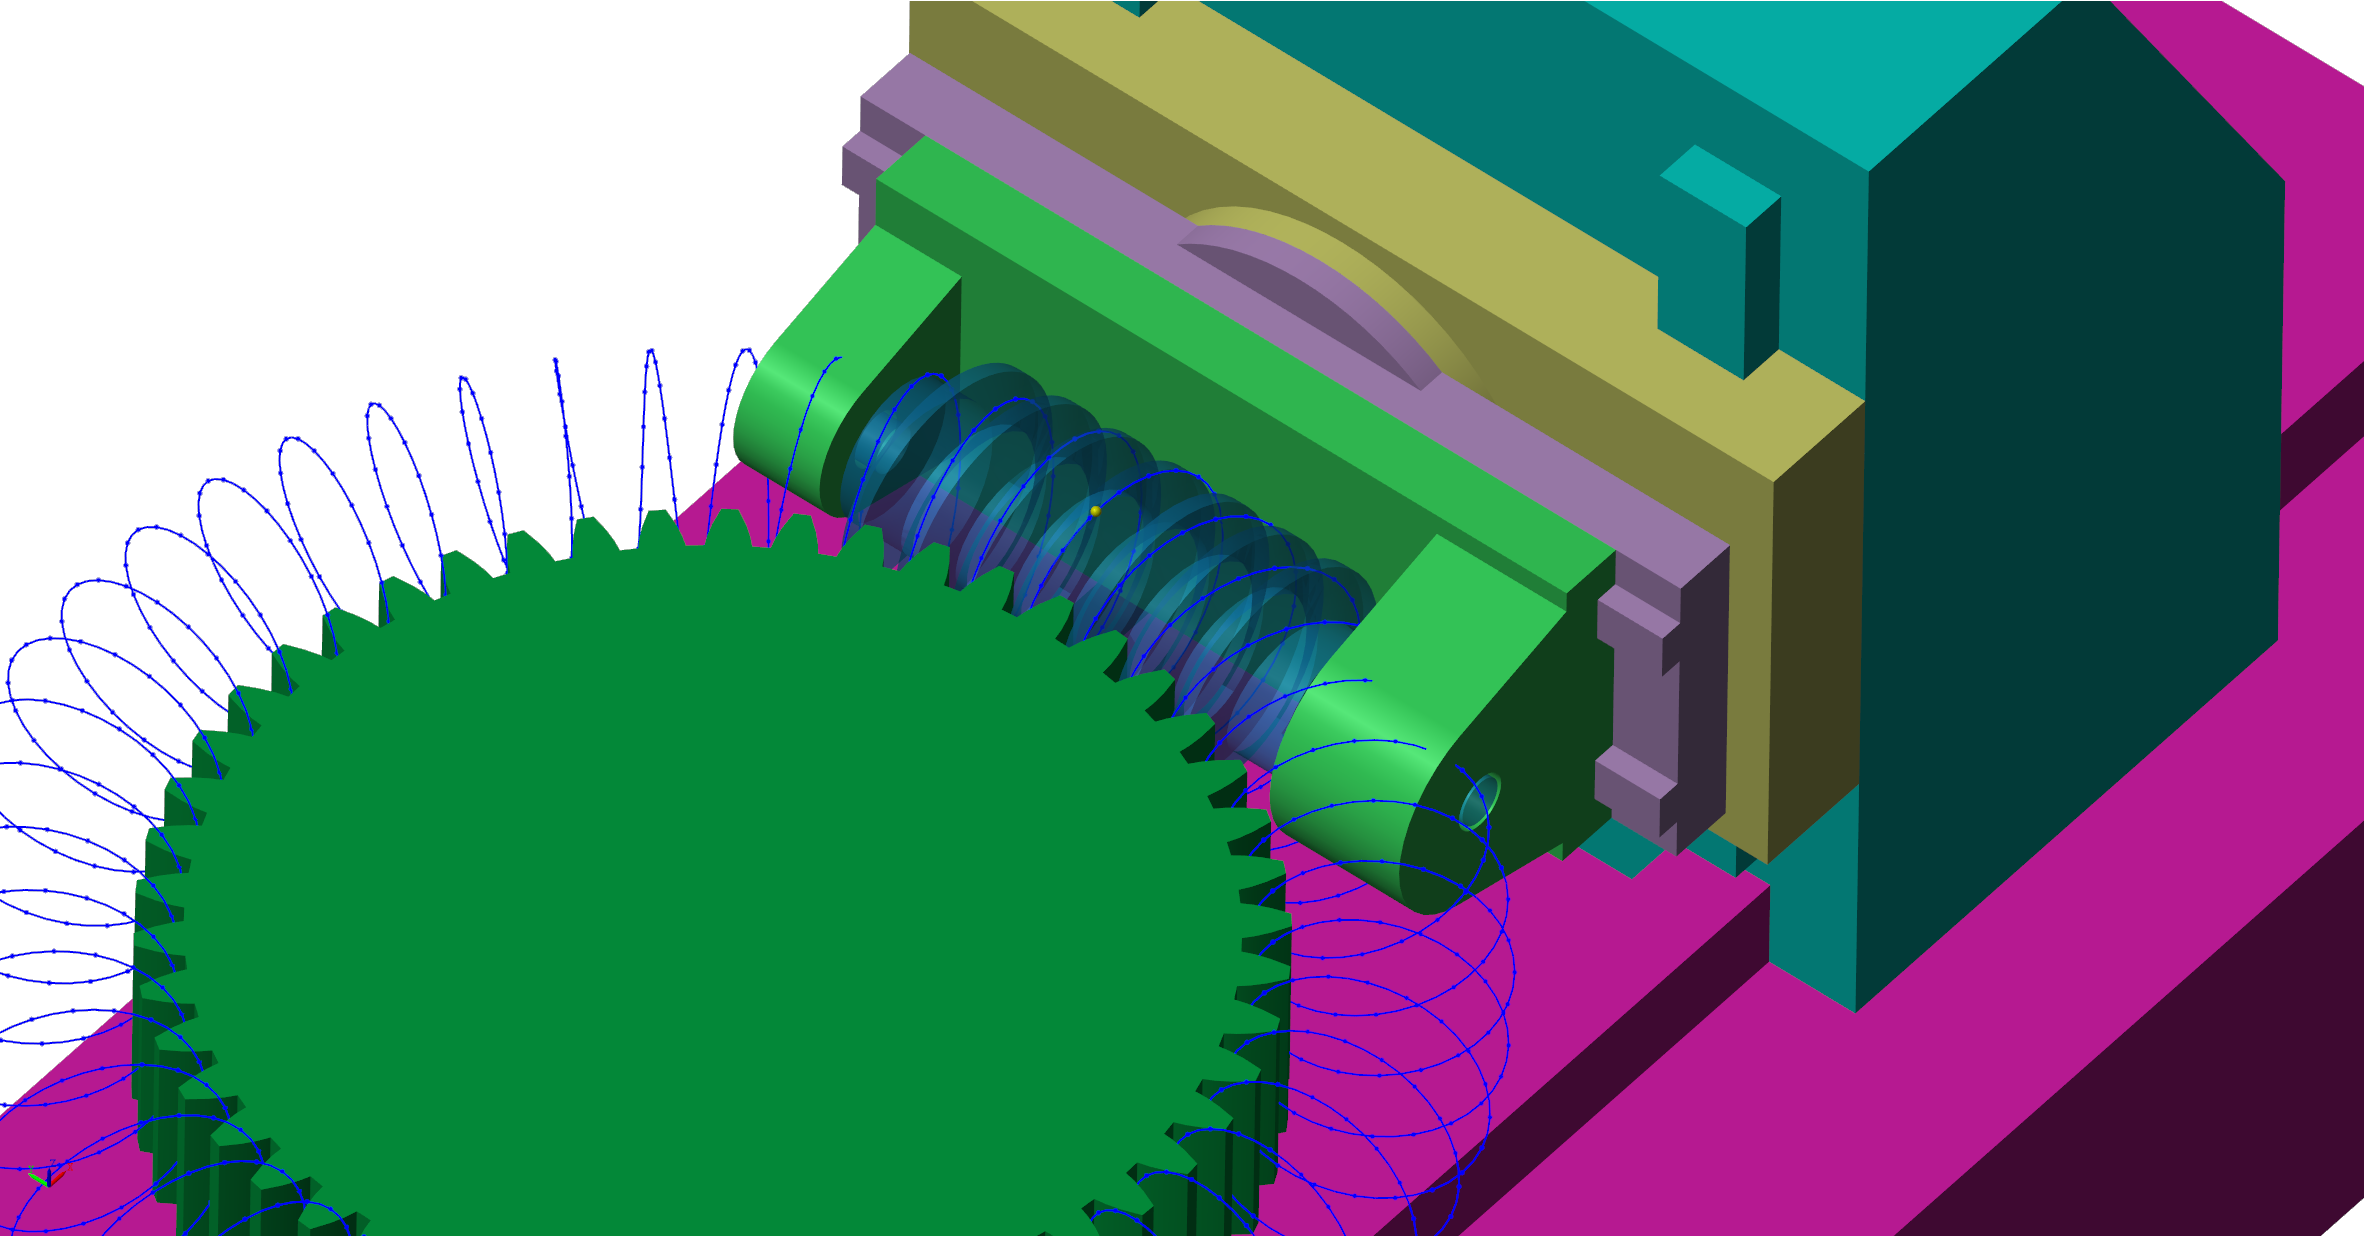
\includegraphics[width=12cm]{mechexplorer}
	\caption{Ausgabe des \simscape Modells im Mechanics Explorer}
	\label{fig:mechexplorer}
\end{figure}

Diese Darstellung ist eine erste und sehr intuitive Visualisierung der Ergebnisse.
Das Ergebnis der linearen Algebra und die \simscape Methode stimmt dann über ein, wenn sich das Frame des PoI entlang der berechneten Trajektorie bewegt.
Zwar kann in der grafischen Ausgabe die Sichtbarkeit der Frames eingestellt werden, die Anzeige wird jedoch schnell unübersichtlich.
Deshalb wurde die Position des PoI durch Einhängen eines Sphere Solid Blocks in einer auffälligen Farbe markiert.

Durch eine Abweichung des PoIs von der Trajektorie kann ein systematischer Fehler direkt erkannt und eine einfache Fehlersuche betrieben werden.
So konnte beispielsweise festgestellt werden, dass zu Beginn der Entwicklung der linearen Algebra die Reihenfolge bei Definition der Werkzeugkoordinaten inkorrekt war.
Ursprünglich war ein Punkt in Werkzeugkoordinaten folgendermaßen definiert:

\begin{equation*}
	\vec{p}_\mathrm{Wz,kart} = \begin{pmatrix} x \\ y \\ z \end{pmatrix}
								= \begin{pmatrix} r \cdot \cos{\phi}\\ h \\ r \cdot \sin{\phi}\end{pmatrix}
\end{equation*}

Allerdings war eine Abweichung des PoIs von der Trajektorie zu erkennen.
Diese verschwand nur als die Reihenfolge beim Einlesen der Koordinaten für die Transformation des PoI vertauscht wurde.
Es war somit klar, dass das Werkzeug ein Koordinatensystem mit z-Achse in Richtung der Rotationsachse benötigt, damit, wie in Abbildung \ref{fig:hobspindle_coord} gezeigt, das Polar- und kartesische Koordinatensystem vorteilhaft aufeinander liegen.
So ergab sich die Definition der Werkzeugkoordinaten gemäß Gleichung \ref{eq:wkzgkoord}.

\begin{figure}
	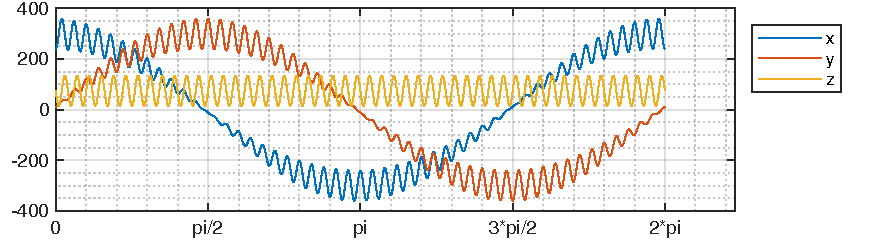
\includegraphics{koordkomps}
	\caption[Komponenten der Trajektorien-Koordinaten]{Komponenten der Trajektorien-Koordinaten aufgetragen gegen den Winkel des Werkstückes}
	\label{fig:koordkomps}
\end{figure}

Im nächsten Schritt werden die Koordinaten der erzeugten Trajektorien analysiert.
Es bietet sich an, die Daten wie in Abb. \ref{fig:koordkomps} gegen den Winkel des Werkstückes aufzutragen, da sich Fehler typischerweise periodisch mit der Werkstückumdrehung gezeigt haben.
Um ein grundsätzliches Verständnis dafür zu bekommen, wie sich beide Methoden zueinander verhalten, bot es sich an den Abstand $d$ der respektiven Punkte auf den Bahnen zu jedem Zeitpunkt anzusehen.
Der Abstand der Punkte beider Trajektorien wird als euklidische Norm berechnet:

\begin{figure}[h]
	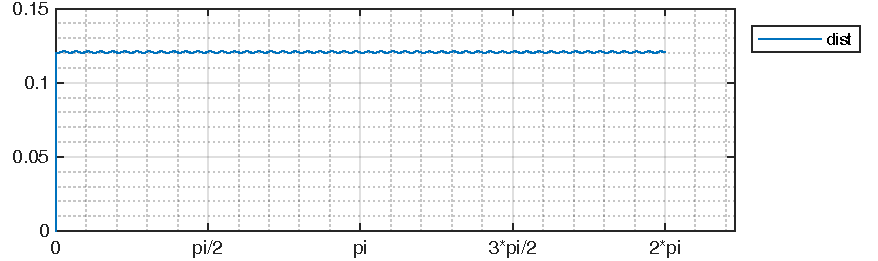
\includegraphics{koorddist}
	\caption[Abweichung der Methoden]{Abweichung der Methoden zueinander gegen den Werkstückwinkel}
	\label{fig:koorddist}
\end{figure}

\begin{equation*}
	d = \sqrt{\left(x_2-x_1\right)^2 + \left(y_2-y_1\right)^2 + \left(z_2-z_1\right)^2}
\end{equation*}

Dieser Abstand wird ebenfalls über den Winkel des Werkzeugs aufgetragen, und ist null wenn sich beide Methoden gleich verhalten.
Man stellt allerdings fest, dass sich eine bleibende Abweichung einstellt, auch wenn die Lösungen grundsätzlich übereinstimmen (vgl. Abb. \ref{fig:koorddist}).
Die genau Ursache für diese Abweichung wurde nicht ausfindig gemacht.
Es wird allerdings vermutet, dass es sich um eine Überlagerung von Ungenauigkeiten beider Methoden handelt.

Dafür spricht, dass der Fehler augenscheinlich die gleiche Frequenz wie die Plots der Koordinatenkompenten hat.
Außerdem ändert sich der Wert um den der Fehler schwingt nicht mit dem Werkstückwinkel.
Das selbe Verhalten zeigt sich bei einer Analyse der Abweichung je Komponente anhand Abb. \ref{fig:xkomps}, wobei hier noch eine tieferfrequente Funktion überlagert zu sein scheint.
Die Frequenz dieser überlagerten Funktion entspricht wohl der Kreisfrequenz des Werkstückes.

\begin{figure}
	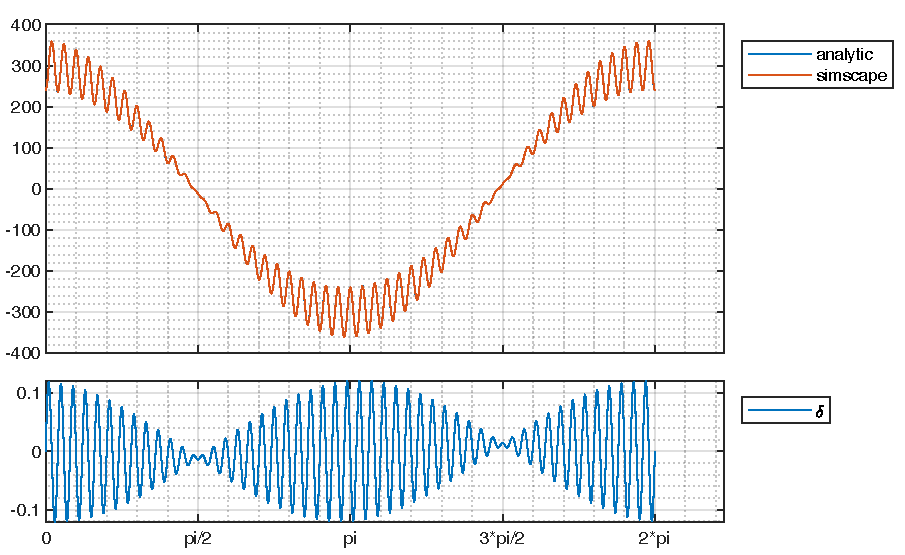
\includegraphics{xkomps}
	\caption[Fehler der x-Komponenten]{x-Komponenten beider Methoden und respektiver Fehler $\delta$ gegen den Werkstückwinkel}
	\label{fig:xkomps}
\end{figure}

Trotz dieser unerklärten Abweichung ist die Methode geeignet, da nur eine qualitative Aussage gefordert wurde.
